\section{Marco Teorico} 

\begin{itemize}
\subsection{Modelo Dimensional}
	\item Técnica de diseño lógico que busca presentar la información de manera intuitiva. Emplea el modelo relacional con algunas importantes restricciones. Util para resumir y organizar los datos y la presentación de información para soportar el análisis de la misma. Existen algunos conceptos básicos para comprender la filosofía de este tipo de modelado: áreas temas, medidas, dimensiones y hechos.
\\
Existen Diagramas referenciales para poner en practica el modelado dimensional:

\item Estrella
\begin{center}
	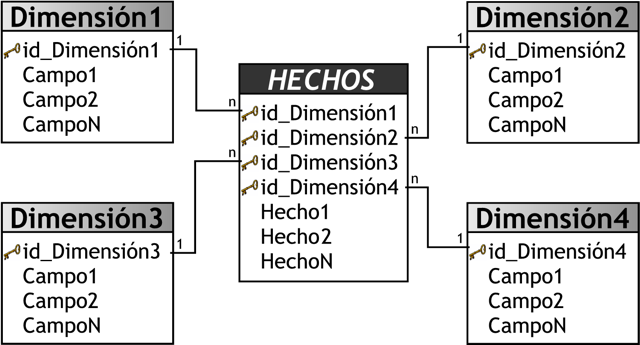
\includegraphics[width=10cm]{./Imagenes/1} 
\end{center}

\item Copo de Nieve
\begin{center}
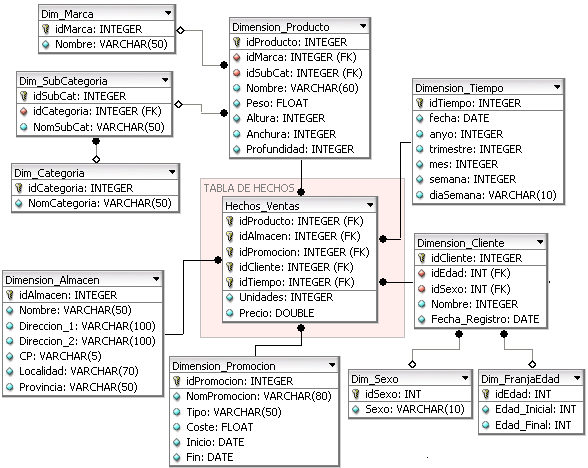
\includegraphics[width=10cm]{./Imagenes/2}
\end{center}


\item Constelacion
\begin{center}
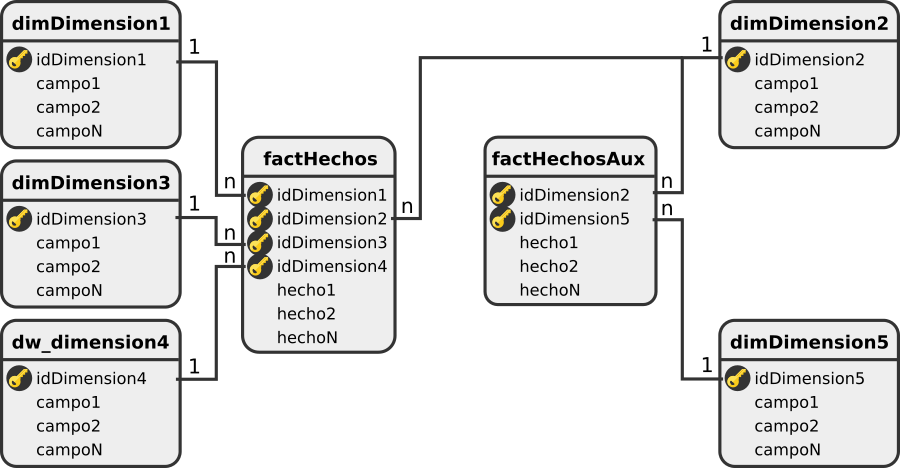
\includegraphics[width=10cm]{./Imagenes/3}
\end{center}

\subsection{Modelo Tabular}
	\item Los modelos tabular son base de datos de Analysis Services que se ejecutan en memoria o en modo DirectQuery(directo a la fuente). La base de datos que usaremos se descargar desde Github que es WorldWideImportersDW 

Todos los que hayan trabajado en Business Intelligence con las herramientas de Microsoft ya conocen lo que son los proyectos Multidimensionales de bases de datos. Son bases de datos hechas para la generación de reportes con un diseño especial muy diferente a las bases de datos transaccionales y con otro motor de base de datos.
Los modelos tabulares son bases de datos “en memoria” de Analysis Services. Gracias a los algoritmos de compresión avanzados y al procesador de consultas multiproceso, el motor analítico en memoria xVelocity (VertiPaq) ofrece un acceso rápido a los objetos y los datos de los modelos tabulares para aplicaciones cliente de reportes como Microsoft Excel y Microsoft Power View.
Los modelos tabulares admiten el acceso a los datos mediante dos modos: modo de almacenamiento en caché y modo DirectQuery. En el modo de almacenamiento en caché, puede integrar datos de varios orígenes como bases de datos relacionales, fuentes de distribución de datos y archivos de texto planos. En el modo DirectQuery, puede omitir el modelo en memoria, lo que permite a las aplicaciones cliente consultar los datos directamente en el origen relacional (SQL Server).
Analysis Services proporciona funciones de procesamiento analítico en línea (OLAP) y minería de datos para aplicaciones de Business Intelligence.
Los proyectos multidimensionales si bien les falta mucho para poder ser tan estables como las bases de datos transaccionales, están en una etapa más avanzada de desarrollo y grandes empresas ya lo utilizan.

Sugerencias:

\item  Primeramente, si ya se tiene una base de datos multidimensional, no se recomienda moverse a base de datos tabulares.
\item El hardware requerido para un proyecto tabular es muy diferente al requerido por un proyecto multidimensional. Por la compresión de datos, requiere menos disco una modelo tabular, pero requiere mucha más memoria RAM porque todo lo usa en memoria. En general, se necesita un buen CPU y memoria.
\item Los modelos tabulares consumen muchos recursos, por lo que se recomienda hacer pruebas del funcionamiento en un servidor de desarrollo y no en producción.
\item Se puede tener un modelo tabular y uno multidimensional instalados en la misma máquina, pero no es recomendable hacerlo en producción.

Ventajas del modelo tabular:

\item Mucho más veloz en consultas.
\item No requiere generar Aggregations (agregaciones) por lo que se simplifica el tiempo de procesamiento.
\item Gracias al DAX (el lenguaje para acceder a los datos equivalente al MDX), tiene mayor flexibilidad para obtener información.
\item Es intuitivo por lo que es mucho más rápido y fácil de entender e implementar.
\item Se basa en modelos relacionales.

Desventajas del modelo tabular:

\item  Las particiones no se procesaban en paralelo si no secuencialmente, lo que hace que sea más lento el procesamiento.
\item No se pueden usar multiples idiomas.
\item Si son muchos datos tarda bastante en manejar configuraciones de diferentes particiones.
\item El modelo tabular acapara demasiada memoria RAM y a su vez es dependiente de tal que afectará a otras aplicaciones.

Formato transaccional

Los datos transaccionales tienen un registro diferente para cada transacción o elemento. Si un cliente realiza varias compras, por ejemplo, cada una sería un registro diferente, con elementos asociados vinculados por un ID de cliente. Esto a veces se conoce como formato anidado.

\begin{center}
	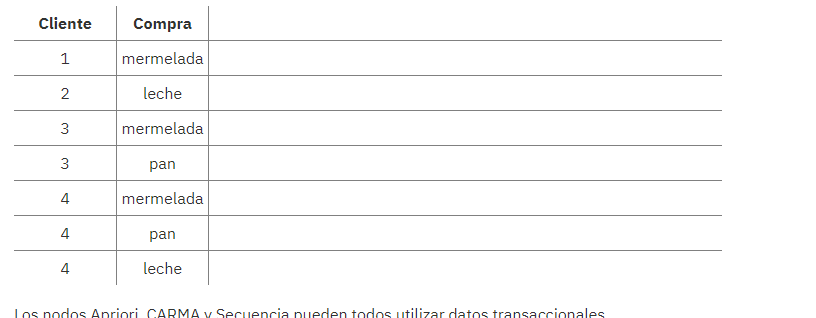
\includegraphics[width=10cm]{./Imagenes/33} 
\end{center}

Datos tabulares

Los datos tabulares (también conocidos como datos de la cesta o de la tabla de verdad) tienen elementos representados por marcadores diferentes, donde cada campo de marcas representa la presencia o ausencia de un elemento específico. Cada registro representa un conjunto completo de elementos asociados. Los campos de marcas pueden ser categóricos o numéricos, aunque ciertos modelos pueden tener requisitos más específicos.

\begin{center}
	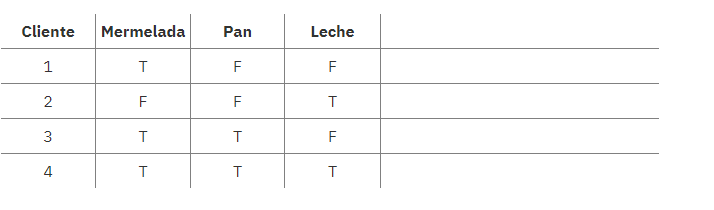
\includegraphics[width=10cm]{./Imagenes/22} 
\end{center}



\end{itemize}